\section{Results}

\begin{table}[h!]\footnotesize
\caption{Settings and performance for the figures}
\begin{tabular}{lllllll}
\hline
Figure & $\vec{u}_{fuel}/\vec{u}_{burnt}$ grid & $T$ grid & $T_{ign}/T_{max}$ & $S$ & $\epsilon_{burnt}$ & Simulation/Rendering time (s) \\
\hline
\ref{fig:fire1}      &	30x60x30	&	90x180x90	&	2200/3000	&	0.1	&		60	&	5/64	\\
\ref{fig:fire2}      &	15x30x15	&	90x180x90	&	2200/3000	&	0.1	&		60	&	3/64	\\
\ref{fig:fire3}      &	60x120x60	&	90x180x90	&	2200/3000	&	0.1	&		60	&	30/64	\\
\ref{fig:fire7}      &	30x60x30	&	90x180x90	&	1500/1500	&	0.1	&		60	&	5/64	\\
\ref{fig:fire8}      &	30x60x30	&	90x180x90	&	2200/3000	&	0.25	&	60	&	5/64	\\
\ref{fig:fire9}      &	30x60x30	&	90x180x90	&	2200/3000	&	0.025	&	60	&	5/64	\\
\ref{fig:fire10}     &	30x60x30	&	90x180x90	&	2200/3000	&	0.1		&	100	&	5/64	\\
\hline
\end{tabular}
\end{table}

Common settings for all figure is $\alpha = 0.15$, $\epsilon_{fuel} = 16/$,  $\rho_{fuel} = 1.0$, $\rho_{burnt} = 0.01$ and $T_{loss} = 3000$. All figures has been rendered on a computer using a Intel 3770K CPU. 

The fire in the figures shown does not consider the walls as boundaries in this simulation and moves therefore through them. The fuel is injected as a sphere in each frame for all but one of the figures.

\begin{figure}[h!]
\centering
\subfigure[frame 9]{\centering

\includegraphics[width=.3 \linewidth]{figures/fire1/9.png}
}
\subfigure[frame 50]{\centering
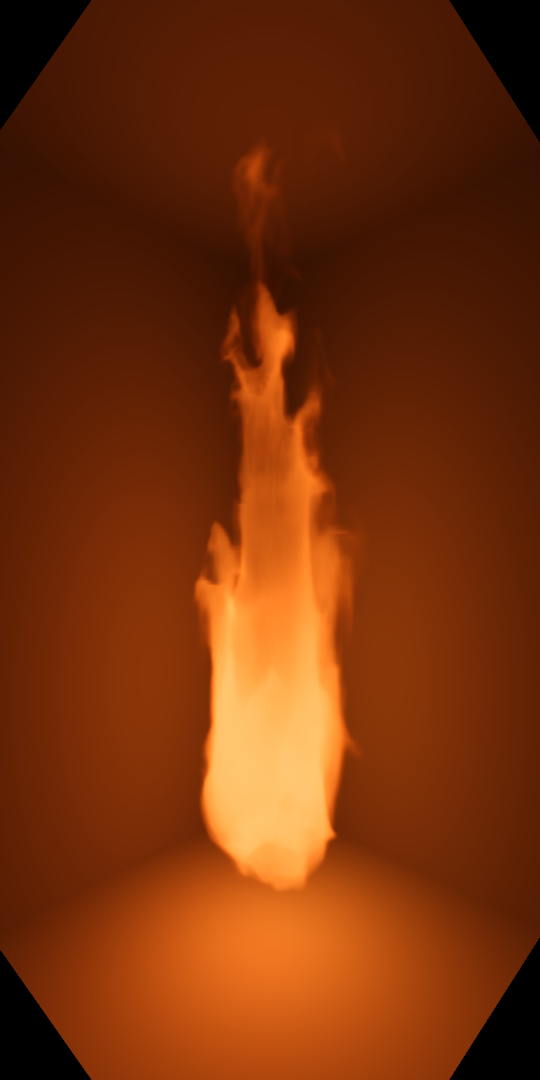
\includegraphics[width=.3\linewidth]{figures/fire1/50.png}
}
\subfigure[frame 144]{\centering
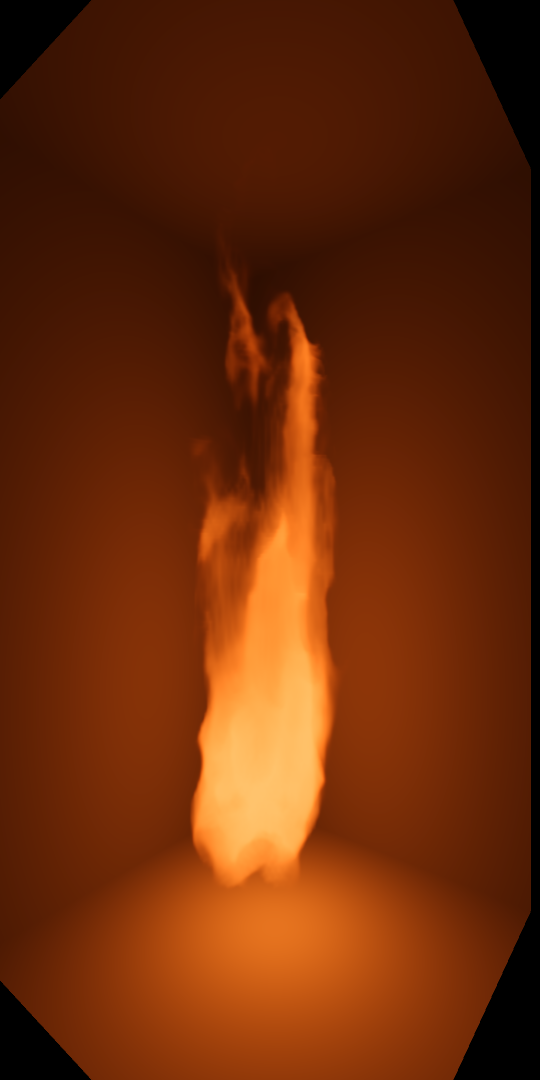
\includegraphics[width=.3\linewidth]{figures/fire1/144.png}
}
\caption
{
\label{fig:fire1}
The figure shows the result of the settings which is used as reference settings for the rest of the figures.
}
\end{figure}

\begin{figure}[h!]
\centering
\subfigure[frame 9]{\centering

\includegraphics[width=.3 \linewidth]{figures/fire2/9.png}
}
\subfigure[frame 50]{\centering
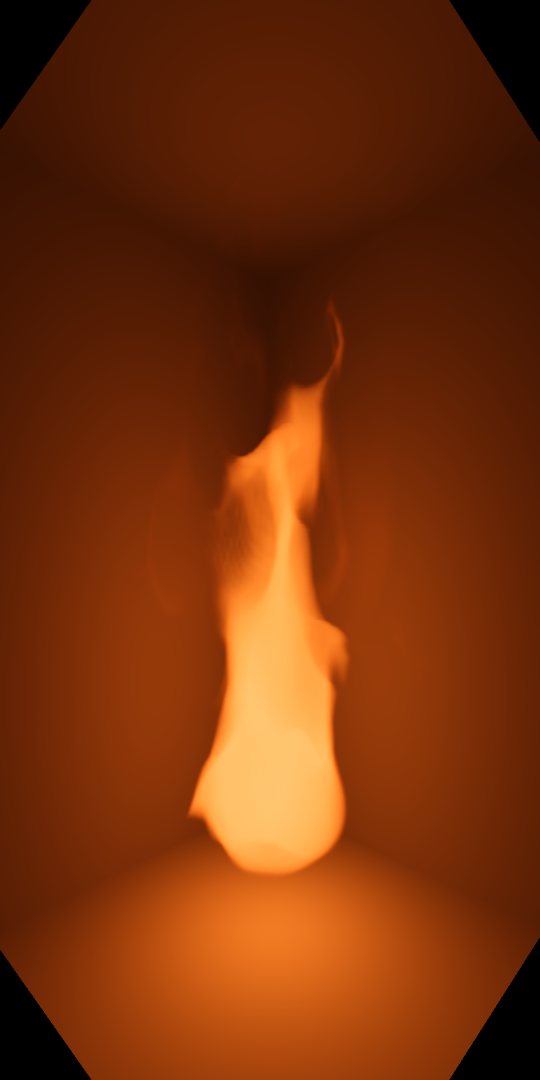
\includegraphics[width=.3\linewidth]{figures/fire2/50.png}
}
\subfigure[frame 144]{\centering
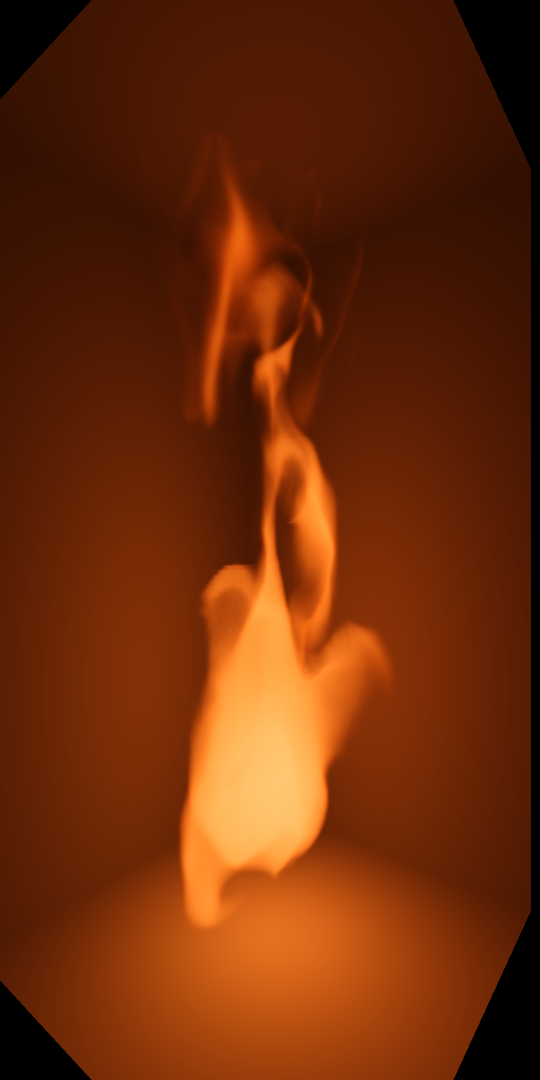
\includegraphics[width=.3\linewidth]{figures/fire2/144.png}
}
\caption
{
\label{fig:fire2}
The velocity grid has half the reference resolution. I.e the simulation has half the resolution.
}
\end{figure} 

\begin{figure}[h!]
\centering
\subfigure[frame 9]{\centering

\includegraphics[width=.3 \linewidth]{figures/fire3/9.png}
}
\subfigure[frame 50]{\centering
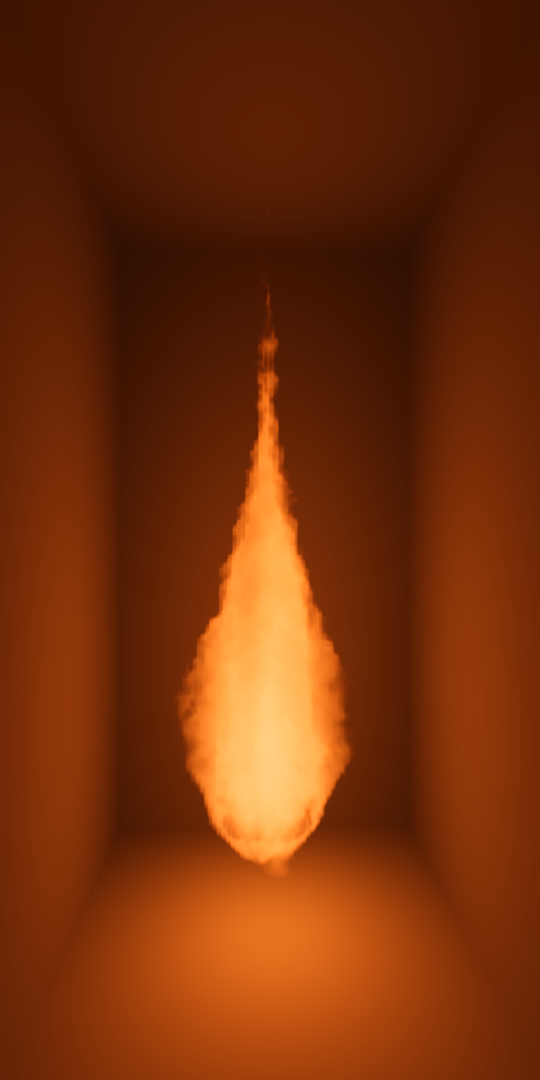
\includegraphics[width=.3\linewidth]{figures/fire3/50.png}
}
\subfigure[frame 144]{\centering
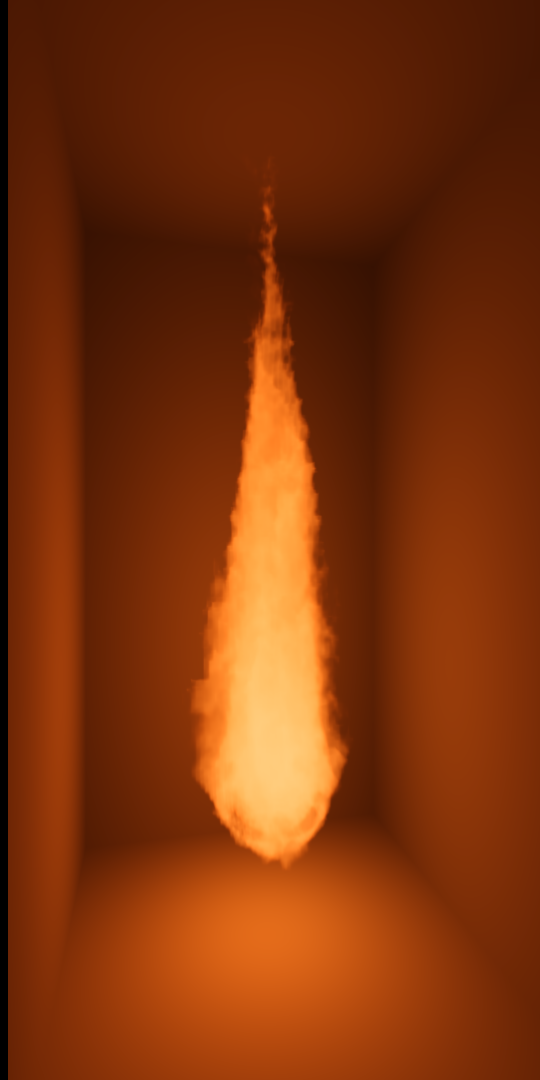
\includegraphics[width=.3\linewidth]{figures/fire3/144.png}
}
\caption
{
\label{fig:fire3}
The velocity grid has twice the reference resolution.
}
\end{figure} 

\begin{figure}[h!]
\centering
\subfigure[frame 9]{\centering

\includegraphics[width=.3 \linewidth]{figures/fire7/9.png}
}
\subfigure[frame 50]{\centering
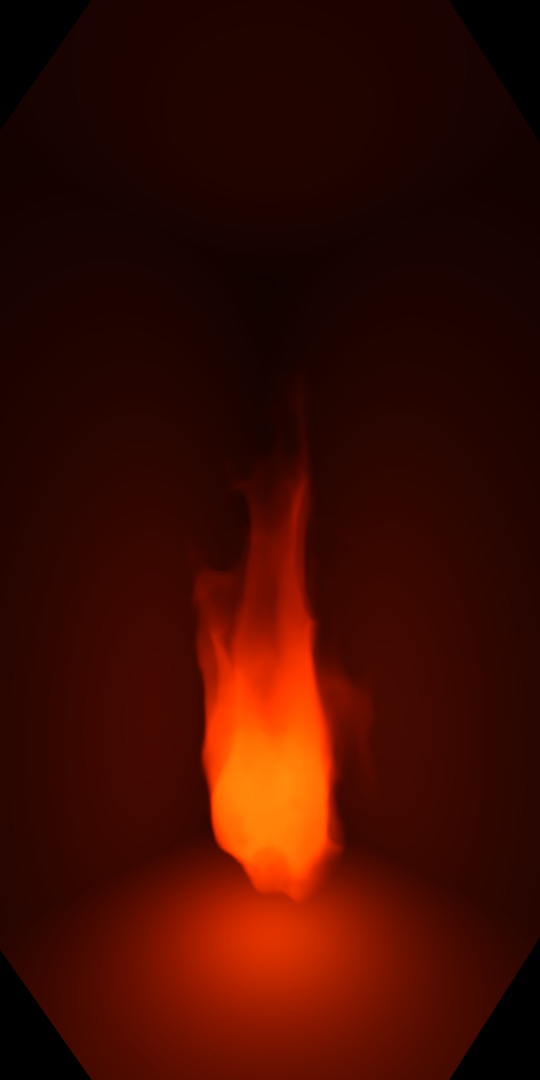
\includegraphics[width=.3\linewidth]{figures/fire7/50.png}
}
\subfigure[frame 144]{\centering
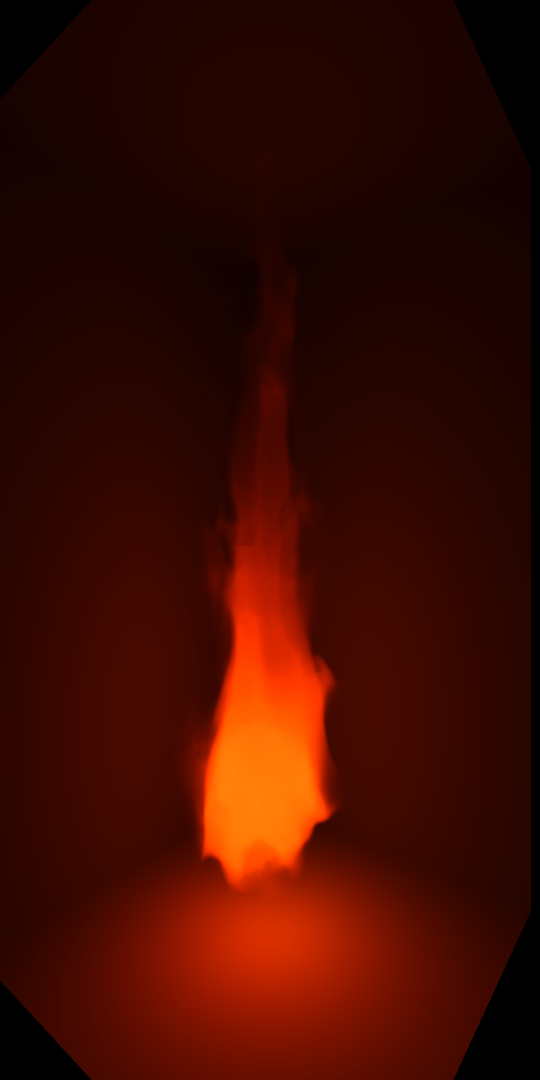
\includegraphics[width=.3\linewidth]{figures/fire7/144.png}
}
\caption
{
\label{fig:fire7}
Using a lower ignition and max temperature than the reference. The chromatic adaptation constant is set to 1 instead of 100.
}
\end{figure} 

\begin{figure}[h!]
\centering
\subfigure[frame 9]{\centering

\includegraphics[width=.3 \linewidth]{figures/fire8/9.png}
}
\subfigure[frame 50]{\centering
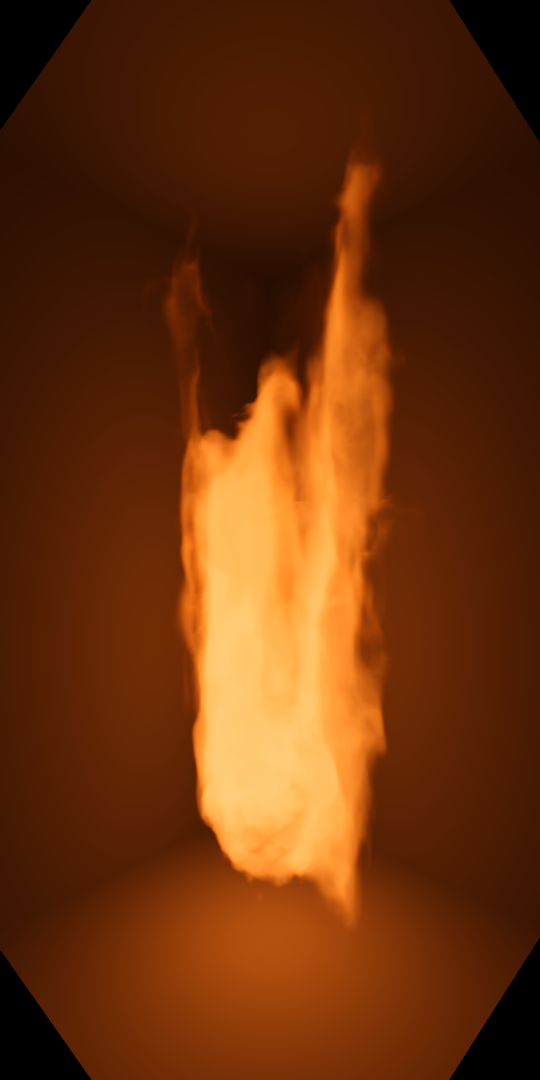
\includegraphics[width=.3\linewidth]{figures/fire8/50.png}
}
\subfigure[frame 144]{\centering
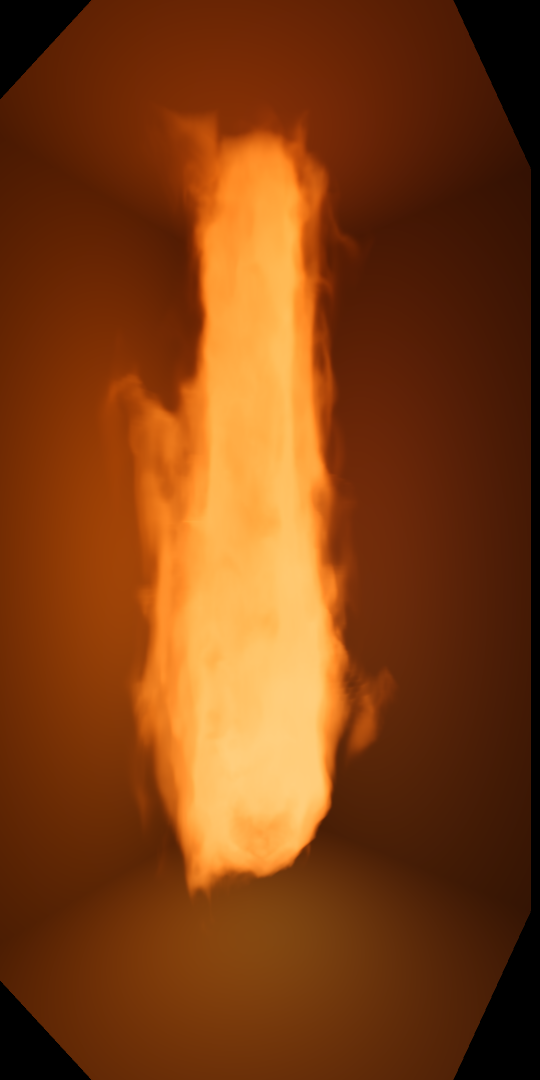
\includegraphics[width=.3\linewidth]{figures/fire8/144.png}
}
\caption
{
\label{fig:fire8}
Using a faster flame speed $S$ than the reference.
}
\end{figure}  

\begin{figure}[h!]
\centering
\subfigure[frame 9]{\centering

\includegraphics[width=.3 \linewidth]{figures/fire9/9.png}
}
\subfigure[frame 50]{\centering
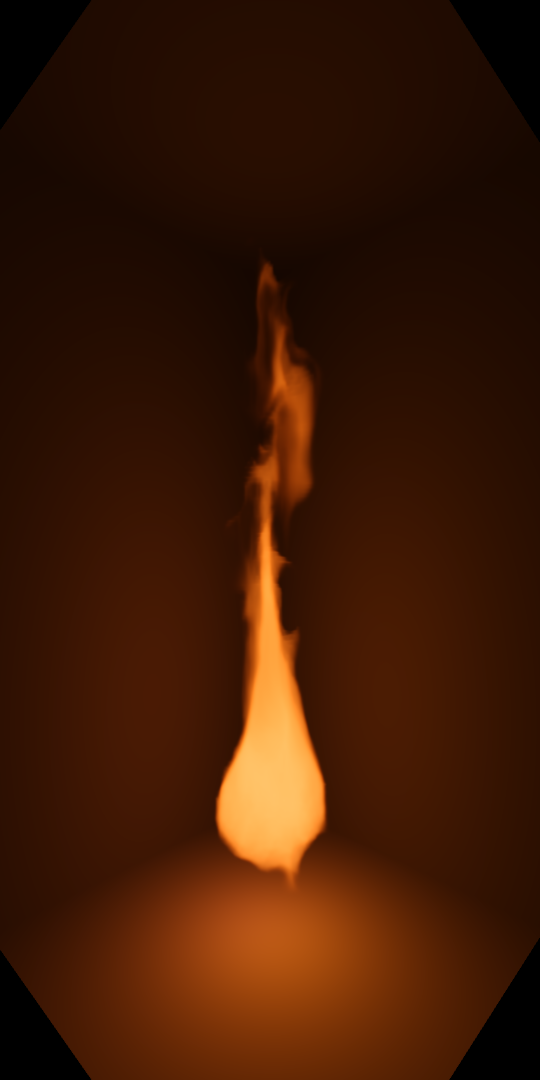
\includegraphics[width=.3\linewidth]{figures/fire9/50.png}
}
\subfigure[frame 144]{\centering
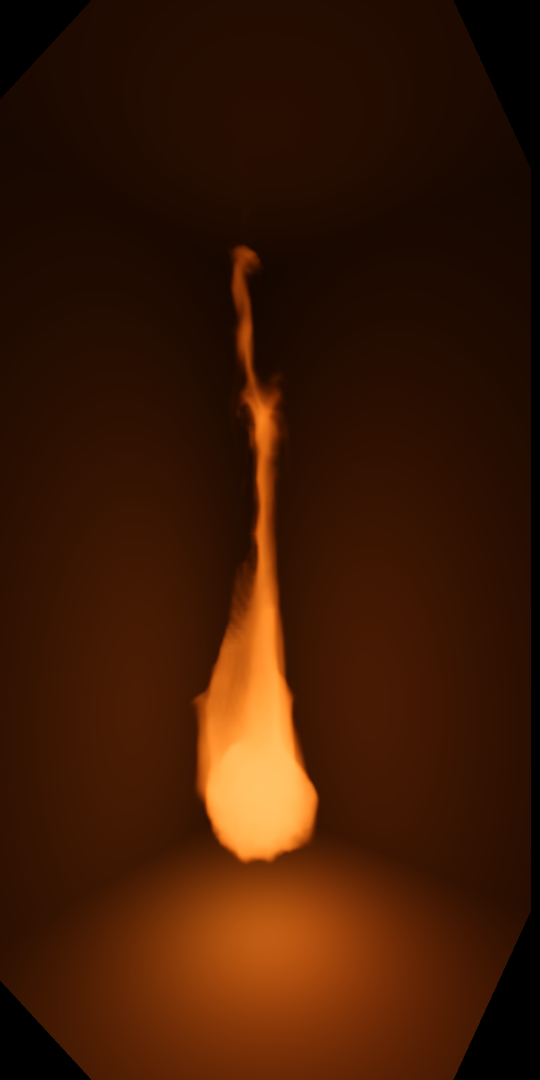
\includegraphics[width=.3\linewidth]{figures/fire9/144.png}
}
\caption
{
\label{fig:fire9}
Using a slower flame speed $S$ than the reference.
}
\end{figure} 

\begin{figure}[h!]
\centering
\subfigure[frame 9]{\centering

\includegraphics[width=.3 \linewidth]{figures/fire10/9.png}
}
\subfigure[frame 50]{\centering
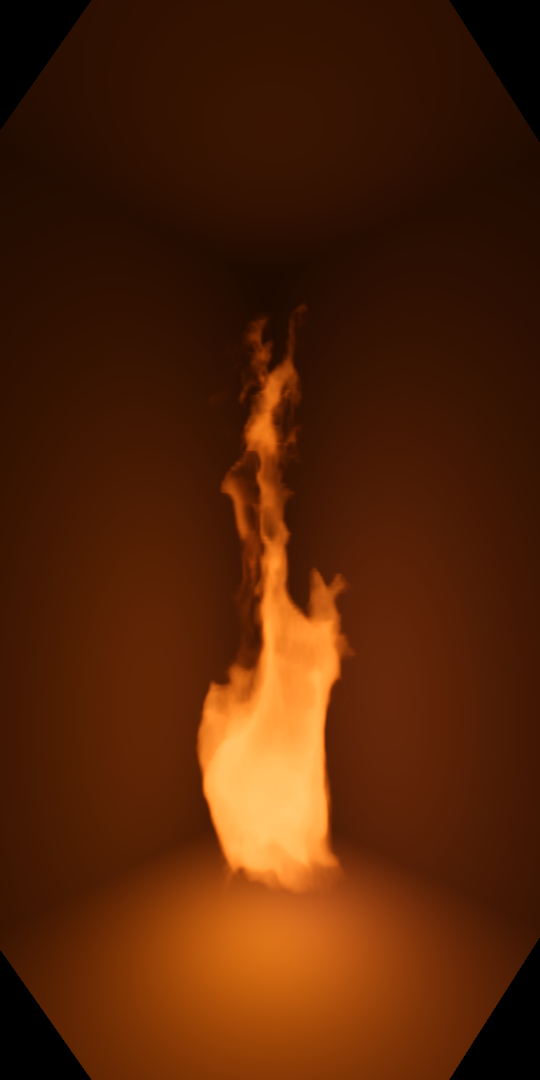
\includegraphics[width=.3\linewidth]{figures/fire10/50.png}
}
\subfigure[frame 144]{\centering
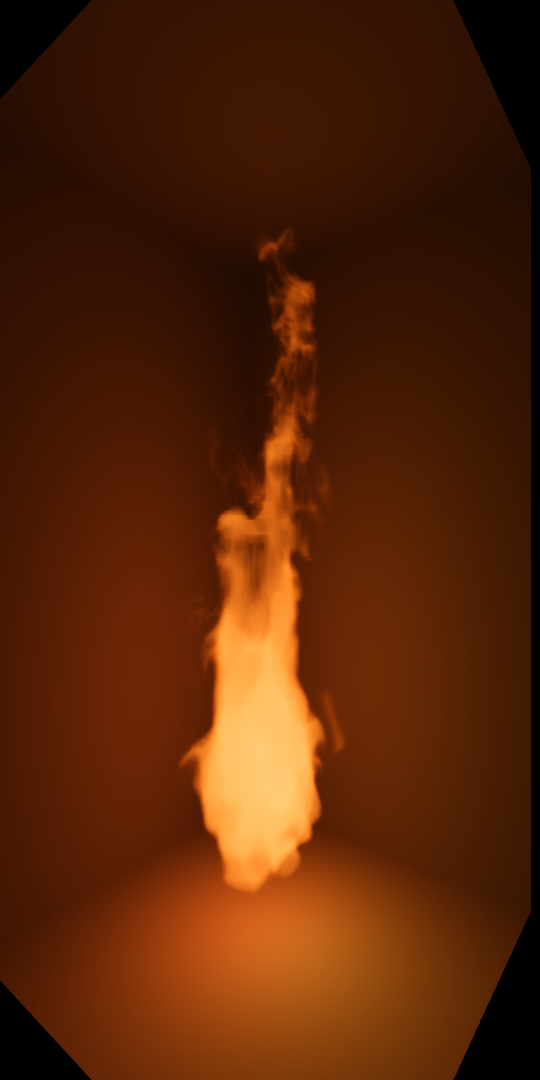
\includegraphics[width=.3\linewidth]{figures/fire10/144.png}
}
\caption
{
\label{fig:fire10}
Using a higher $\epsilon_h$ than the reference.
}
\end{figure} 

\begin{figure}[h!]
\centering
\subfigure[frame 5]{\centering

\includegraphics[width=.3 \linewidth]{figures/fire6/5.png}}
\subfigure[frame 99]{\centering
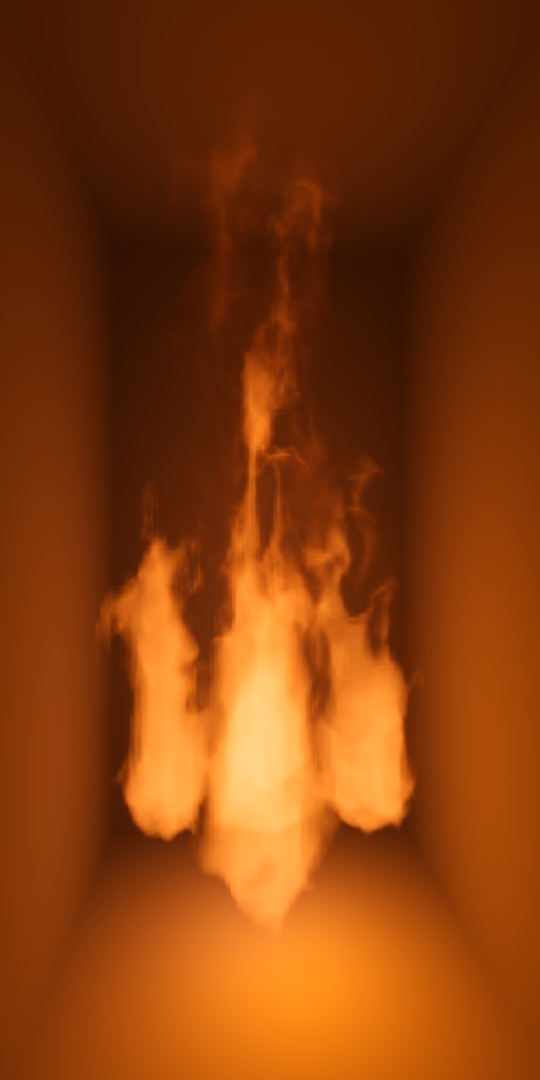
\includegraphics[width=.3\linewidth]{figures/fire6/99.png}}
\caption
{
\label{fig:fire4}
Injecting 5 smaller spheres with fuel instead of one big.
}
\end{figure}  

\begin{figure}[h!]
\centering
\subfigure[frame 9]{\centering

\includegraphics[width=.3 \linewidth]{figures/fire4/9.png}
}
\subfigure[frame 41]{\centering
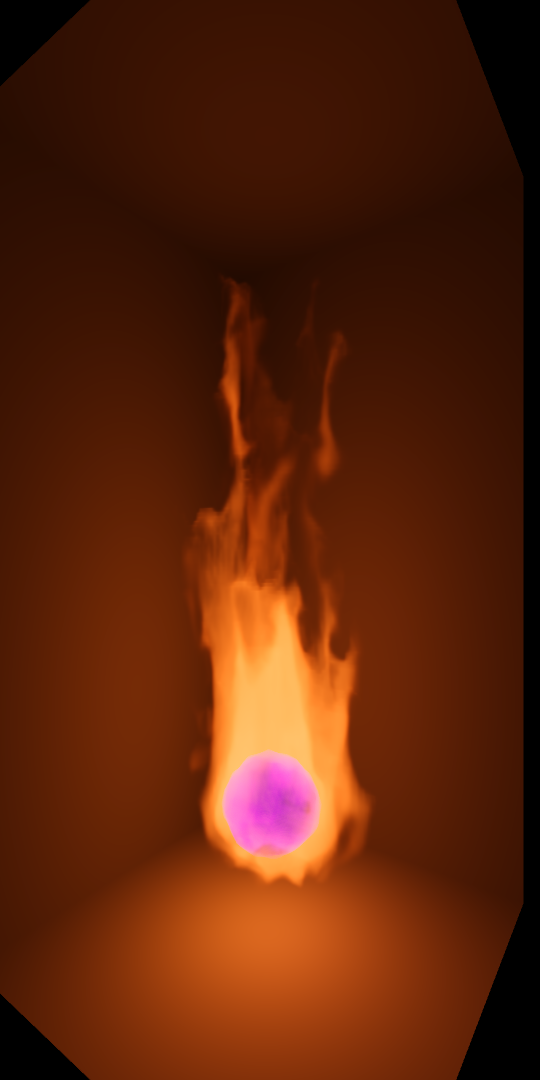
\includegraphics[width=.3\linewidth]{figures/fire4/41.png}
}
\subfigure[frame 50]{\centering
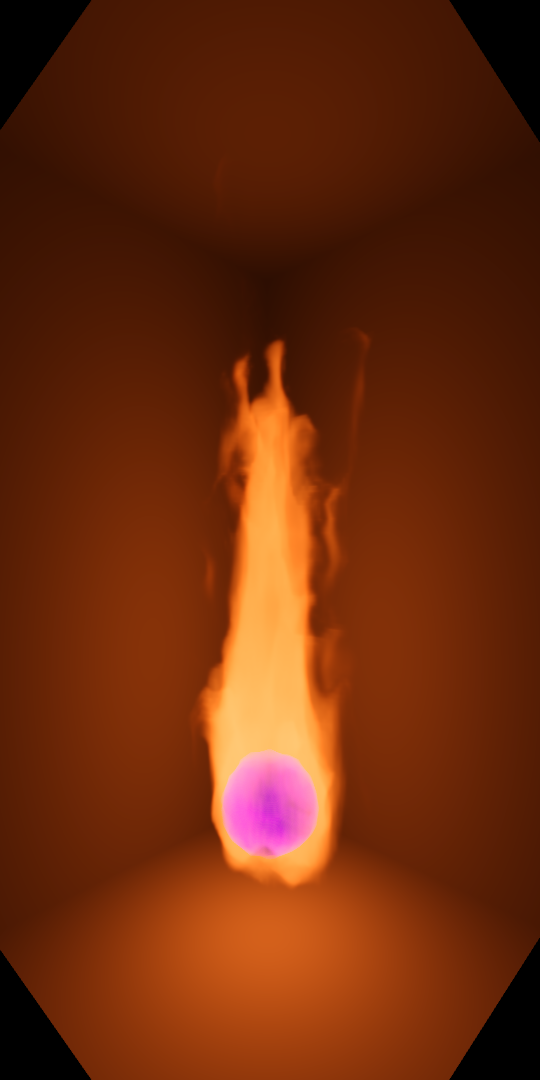
\includegraphics[width=.3\linewidth]{figures/fire4/50.png}
}
\caption
{
\label{fig:fire4}
The blue core convert the radiance from the black body radiation to purple radiance only.   
}
\end{figure}

\begin{figure}[h!]
\centering
\subfigure[frame 2]{\centering
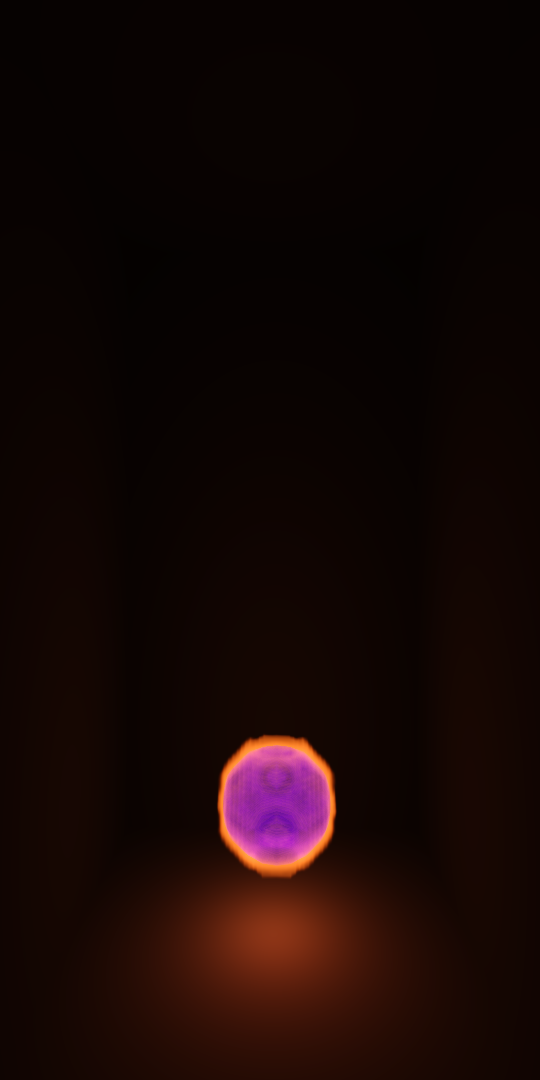
\includegraphics[width=.23 \linewidth]{figures/fire5/2.png}}
\subfigure[frame 9]{\centering

\includegraphics[width=.23\linewidth]{figures/fire5/9.png}}
\subfigure[frame 13]{\centering

\includegraphics[width=.23\linewidth]{figures/fire5/13.png}}
\subfigure[frame 25]{\centering
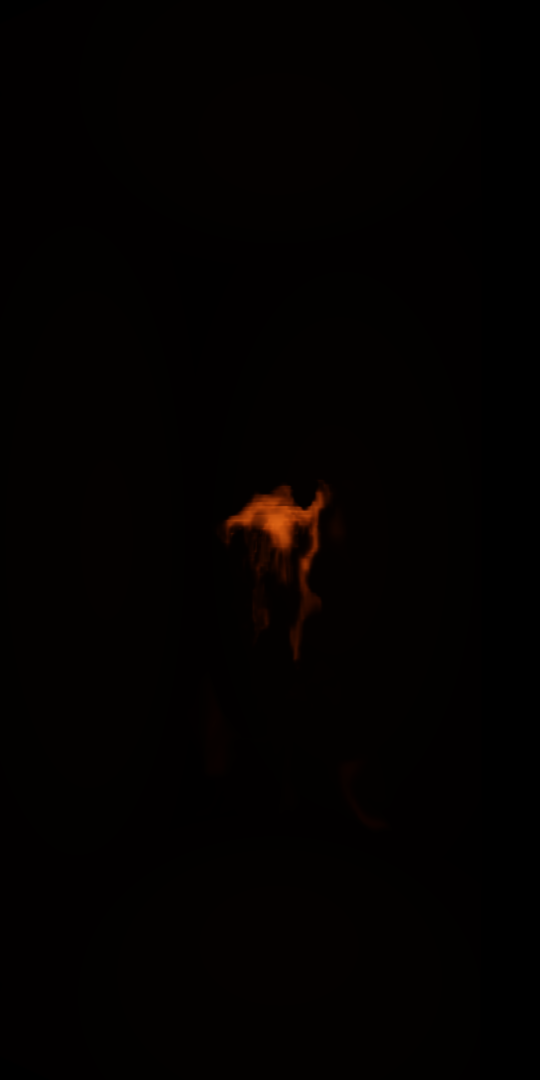
\includegraphics[width=.23\linewidth]{figures/fire5/25.png}}
\caption
{
\label{fig:fire5}
Same as figure \ref{fig:fire5}, but without fuel injection.
}
\end{figure}   

\begin{figure}[h!]
\centering
\subfigure[frame 60]{\centering
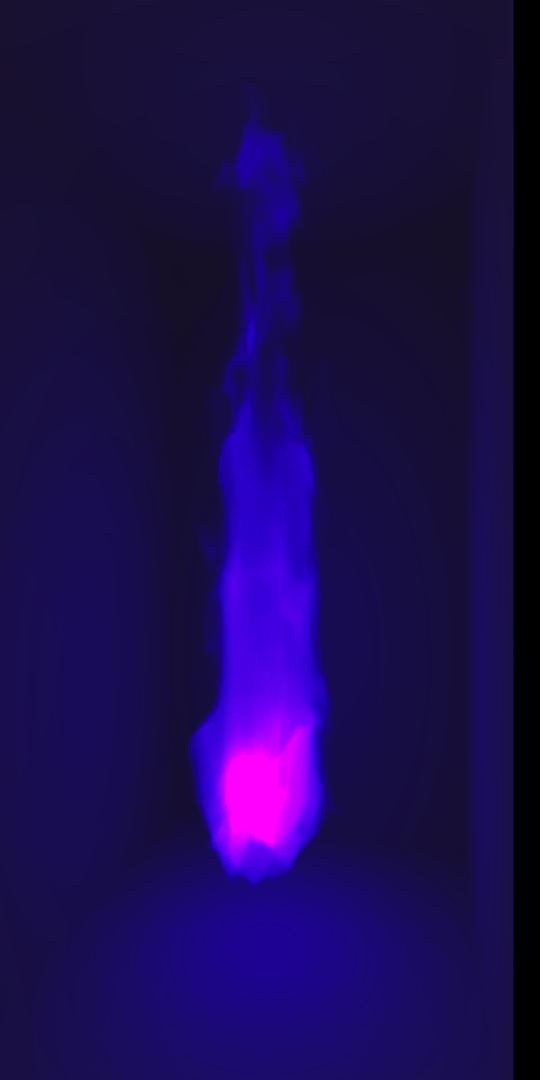
\includegraphics[width=.19 \linewidth]{figures/fire11/60.png}}
\subfigure[frame 68]{\centering
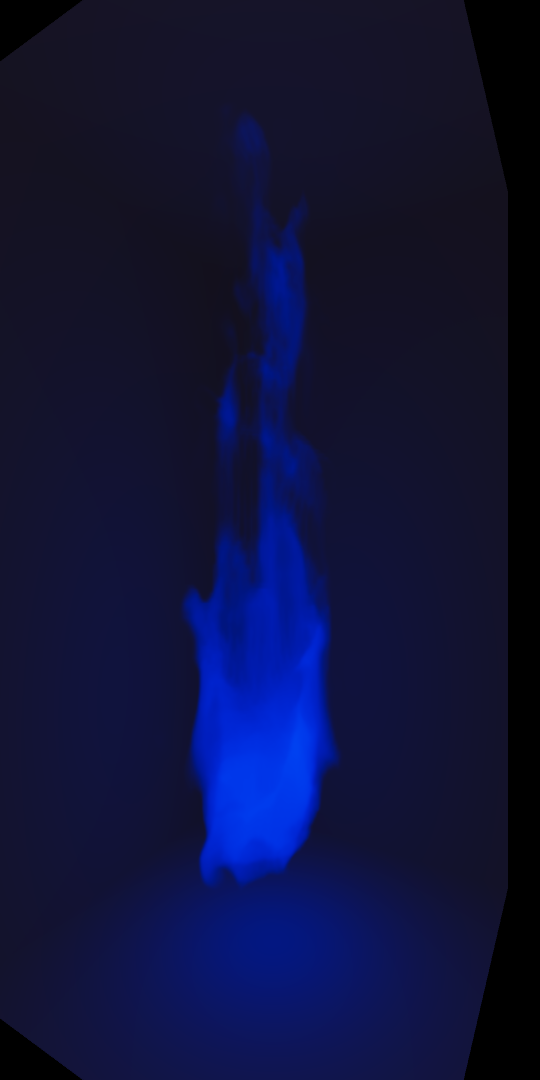
\includegraphics[width=.19\linewidth]{figures/fire11/68.png}}
\subfigure[frame 73]{\centering

\includegraphics[width=.19\linewidth]{figures/fire11/73.png}}
\subfigure[frame 89]{\centering
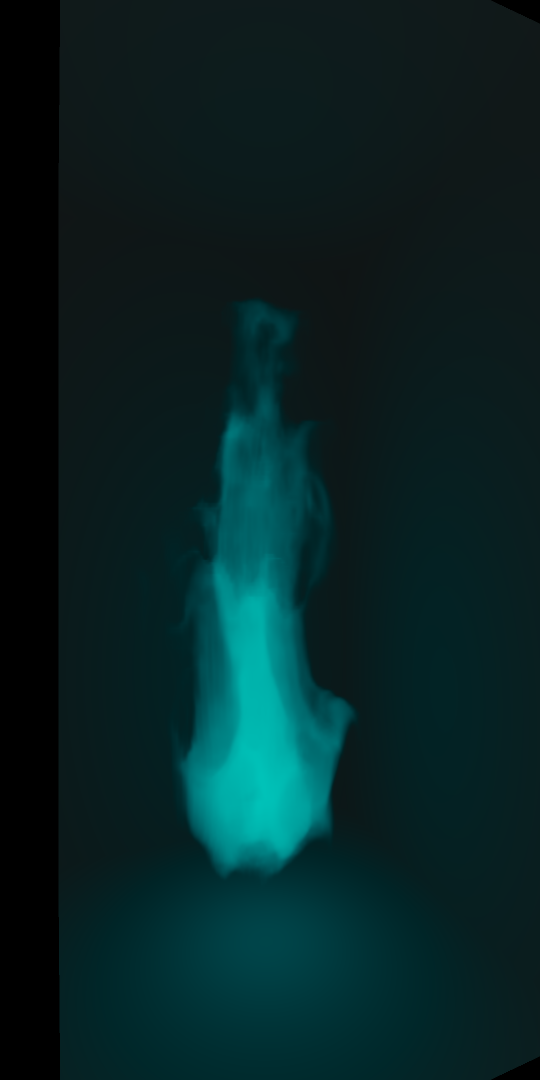
\includegraphics[width=.19\linewidth]{figures/fire11/89.png}}
\subfigure[frame 96]{\centering
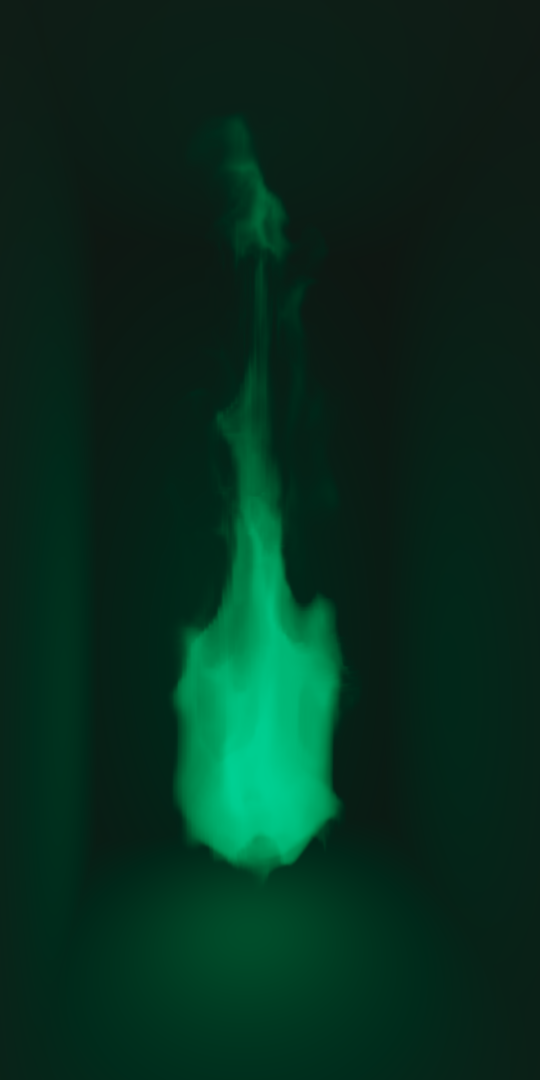
\includegraphics[width=.19\linewidth]{figures/fire11/96.png}}
\subfigure[frame 117]{\centering
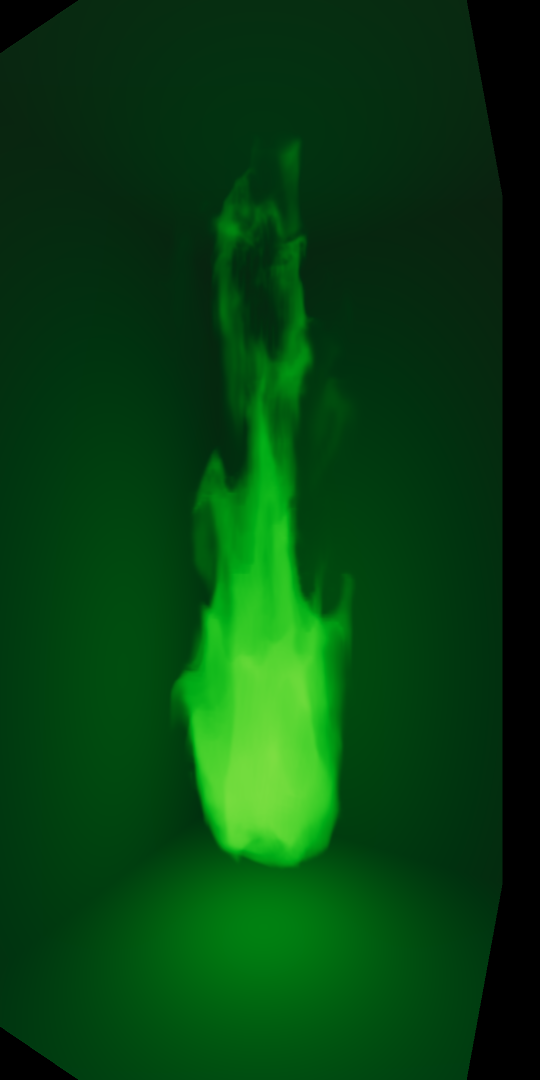
\includegraphics[width=.19\linewidth]{figures/fire11/117.png}}
\subfigure[frame 162]{\centering
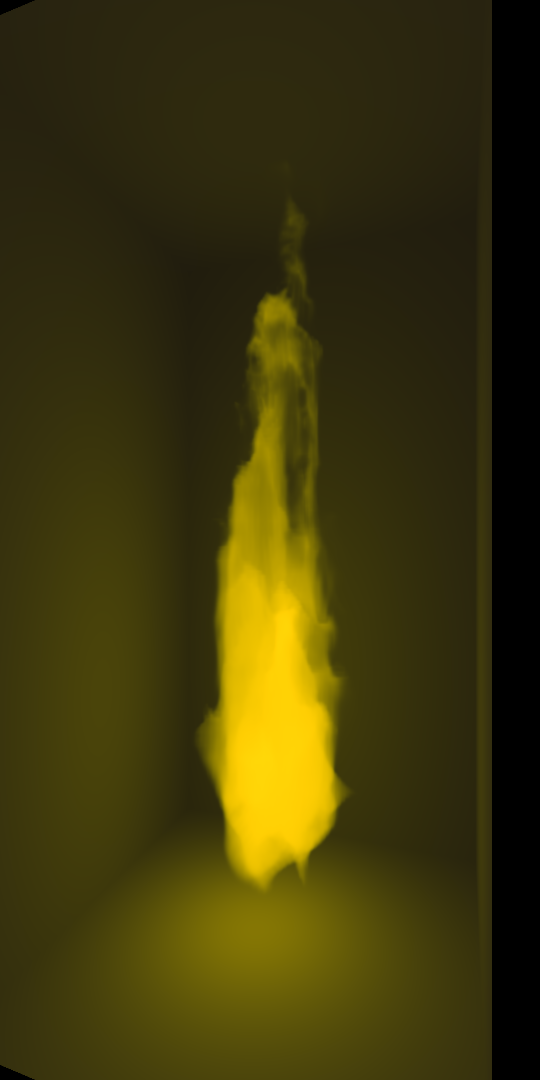
\includegraphics[width=.19\linewidth]{figures/fire11/162.png}}
\subfigure[frame 178]{\centering
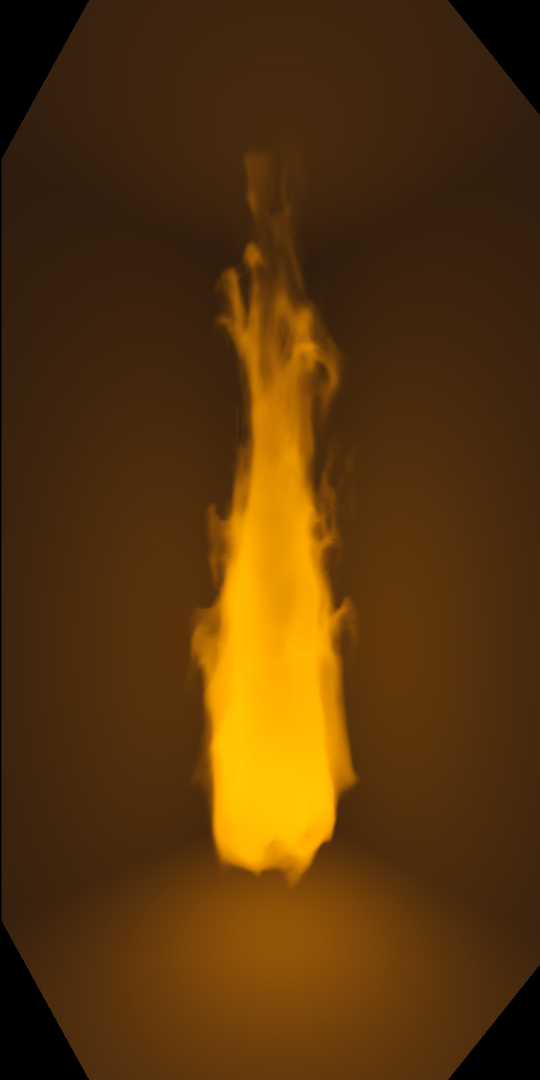
\includegraphics[width=.19\linewidth]{figures/fire11/178.png}}
\subfigure[frame 189]{\centering
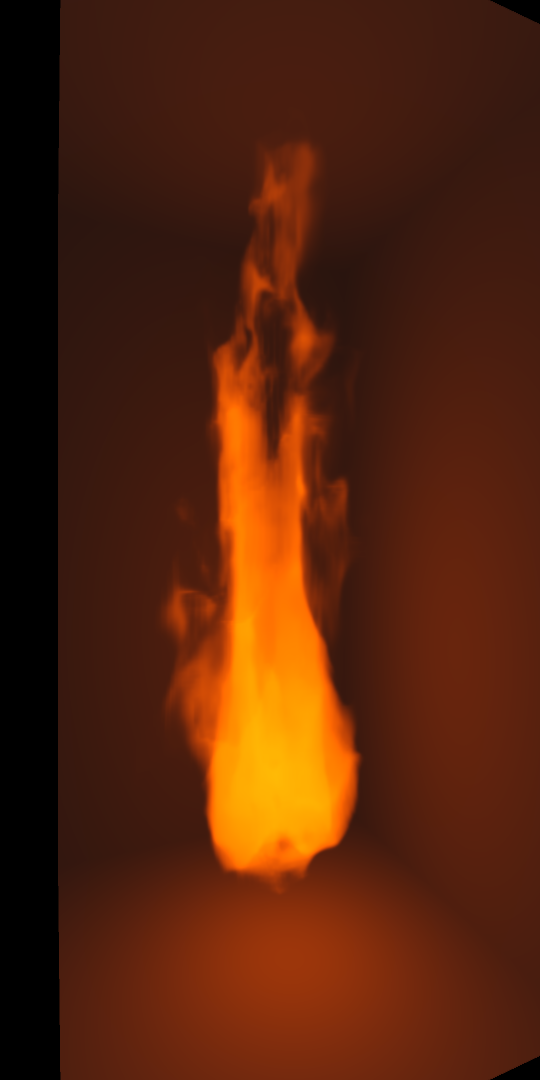
\includegraphics[width=.19\linewidth]{figures/fire11/189.png}}
\subfigure[frame 209]{\centering
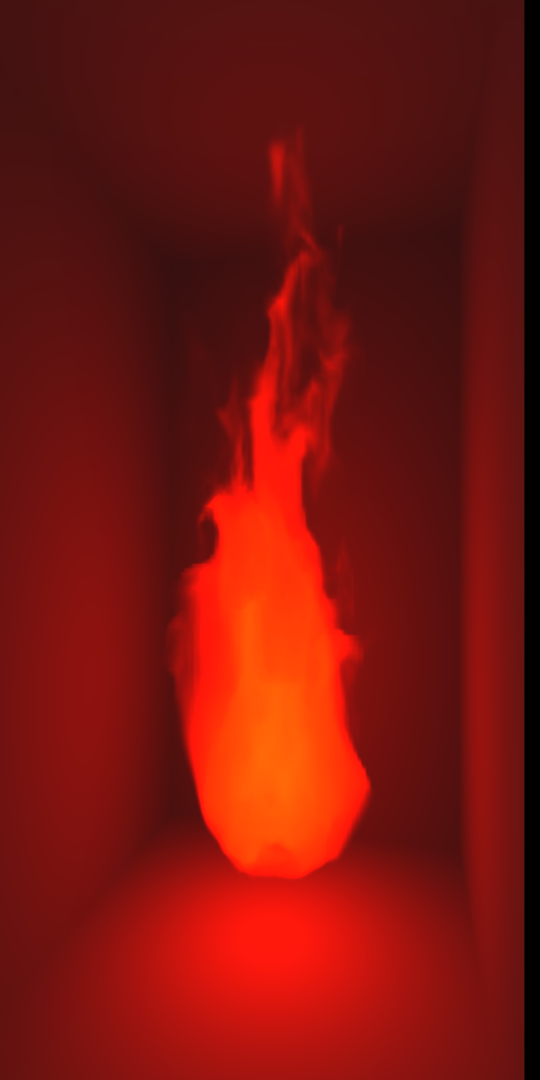
\includegraphics[width=.19\linewidth]{figures/fire11/209.png}}
\caption
{
\label{fig:fire5}
The black body only emits radiance for one wavelength one at the time.
}
\end{figure} 

\begin{figure}[h!]
\centering
\subfigure[frame 4]{\centering
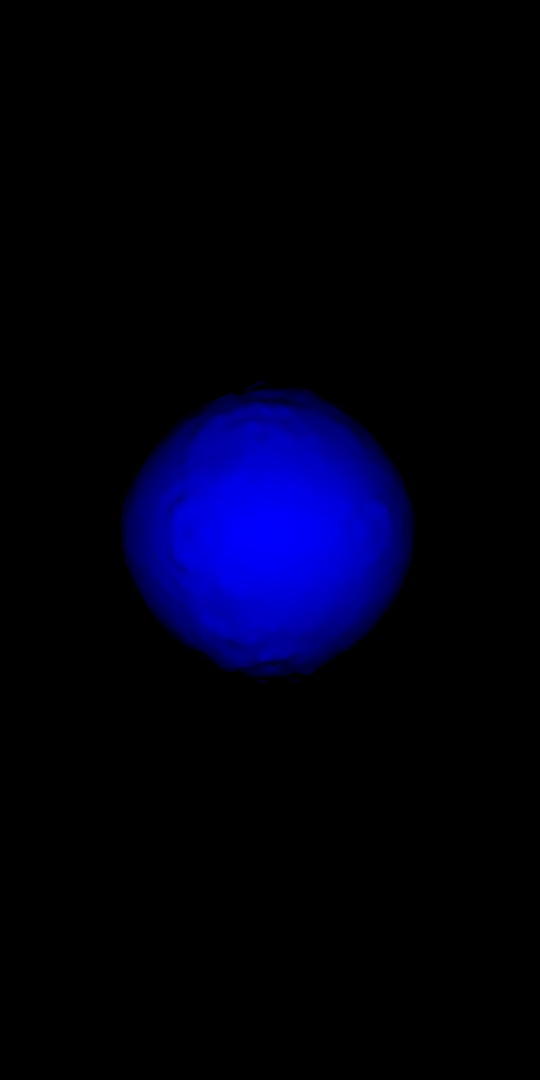
\includegraphics[width=.3 \linewidth]{figures/bluecore/4.png}}
\subfigure[frame 8]{\centering
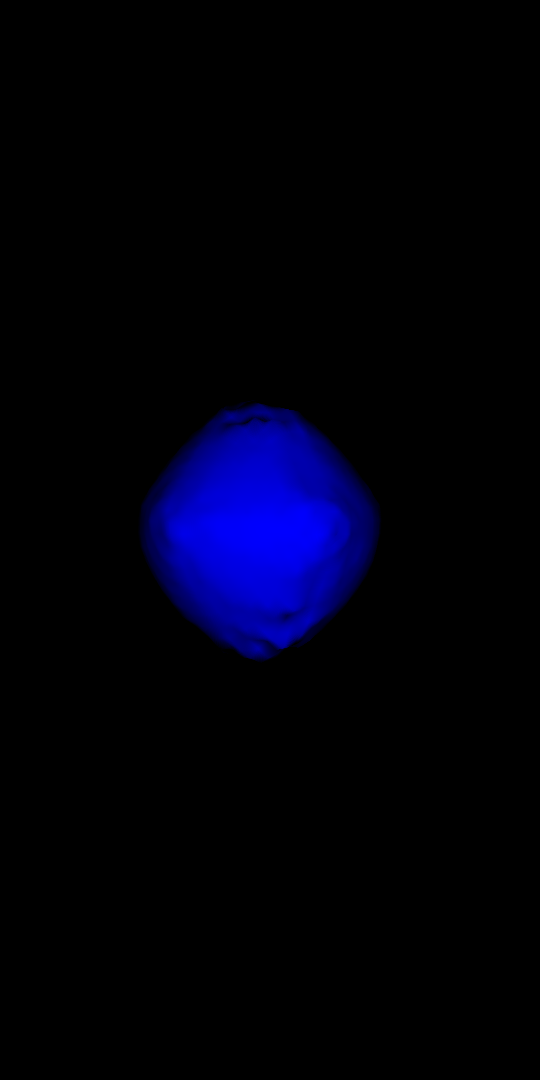
\includegraphics[width=.3\linewidth]{figures/bluecore/8.png}}
\subfigure[frame 20]{\centering

\includegraphics[width=.3\linewidth]{figures/bluecore/20.png}}
\caption
{
\label{fig:fire5}
A burning blue core visualized as a surface.
}
\end{figure}       

Link to a video which demonstrates all the results in the figures:
\href{http://youtu.be/F40\_rowaLQg}{Video link}

